\section{Results and Discussion}
\label{sec:results}

\begin{table*}[t]
\centering
\caption{RadHAR official test recordings (3{,}565 windows, 5 classes). Mean\,$\pm$\,std over 3 seeds. Sig.: number of seeds in which the Holm-corrected McNemar test against the proposed model gives $p<0.05$; $\uparrow$ ours better / $\downarrow$ ours worse. Latency: median, batch 1, one CPU thread.}
\label{tab:radhar}
\setlength{\tabcolsep}{5pt}
\begin{tabular}{lrrrccc}
\toprule
Model & Params (K) & MFLOPs & Lat. (ms) & Accuracy (\%) & Macro-F1 (\%) & Sig. \\
\midrule
Voxel TD-CNN+BiLSTM [RadHAR] & 45.9 & 180.5 & 6.60 & 95.01\,$\pm$\,0.16 & 95.03\,$\pm$\,0.17 & 2/3$\uparrow$ \\
PointNet & 76.2 & 31.8 & 0.74 & 96.31\,$\pm$\,0.66 & 96.36\,$\pm$\,0.64 & 1/3$\uparrow$ \\
PointNet+BiLSTM & 109.1 & 6.6 & 0.83 & 96.14\,$\pm$\,0.23 & 96.16\,$\pm$\,0.21 & 2/3$\uparrow$ \\
PointNet++ (SSG) & 413.4 & 133.1 & 8.44 & 97.34\,$\pm$\,0.18 & 97.37\,$\pm$\,0.19 & 1/3$\downarrow$ \\
DGCNN & 422.4 & 137.9 & 6.95 & 95.85\,$\pm$\,0.00 & 95.89\,$\pm$\,0.00 & 1/3$\uparrow$ \\
Point Transformer & 335.2 & 264.4 & 7.98 & 97.01\,$\pm$\,0.25 & 97.04\,$\pm$\,0.24 & 1/3$\uparrow$ \\
\midrule
STPT-Large (teacher) & 725.3 & 139.5 & 3.59 & 96.44\,$\pm$\,1.43 & 96.48\,$\pm$\,1.42 & 1/3$\uparrow$ \\
STPT-Lite & 117.5 & 36.6 & 2.14 & 96.22\,$\pm$\,1.43 & 96.27\,$\pm$\,1.41 & 2/3$\uparrow$ \\
STPT-Lite + KD & 117.5 & 36.6 & 2.08 & 96.04\,$\pm$\,0.78 & 96.08\,$\pm$\,0.76 & 1/3$\uparrow$ \\
STPT-Tiny + KD & 30.7 & 12.1 & 1.92 & 96.86\,$\pm$\,0.17 & 96.90\,$\pm$\,0.16 & 1/3$\uparrow$ \\
\textbf{STPT-Lite + KD + robust (ours)} & 117.5 & 36.6 & 2.58 & 96.83\,$\pm$\,0.69 & 96.88\,$\pm$\,0.68 & -- \\
PointNet + noise-robust training & 76.2 & 31.8 & 0.73 & \textbf{97.38\,$\pm$\,0.11} & \textbf{97.40\,$\pm$\,0.11} & 1/3$\downarrow$ \\
\bottomrule
\end{tabular}
\end{table*}
\begin{table*}[t]
\centering
\caption{MiliPoint, subject-disjoint test (subjects 8--10, 3{,}569 windows, 49 actions). Same conventions as Table~\ref{tab:radhar}.}
\label{tab:milipoint}
\setlength{\tabcolsep}{5pt}
\begin{tabular}{lrrrccrc}
\toprule
Model & Params (K) & MFLOPs & Lat. (ms) & Accuracy (\%) & Macro-F1 (\%) & Top-3 & Sig. \\
\midrule
PointNet & 81.9 & 31.8 & 0.74 & 32.57\,$\pm$\,4.59 & 29.72\,$\pm$\,4.50 & 59.5 & 3/3$\uparrow$ \\
PointNet+BiLSTM & 114.8 & 6.6 & 0.74 & 28.11\,$\pm$\,4.06 & 28.09\,$\pm$\,4.66 & 56.1 & 3/3$\uparrow$ \\
PointNet++ (SSG) & 424.7 & 133.1 & 7.94 & 8.07\,$\pm$\,5.47 & 5.12\,$\pm$\,5.76 & 21.4 & 3/3$\uparrow$ \\
STPT-Large (teacher) & 730.9 & 139.5 & 3.65 & \textbf{50.39\,$\pm$\,1.39} & \textbf{50.84\,$\pm$\,2.11} & 75.8 & 1/3$\uparrow$ \\
STPT-Lite & 120.4 & 36.6 & 2.60 & 45.79\,$\pm$\,6.30 & 45.95\,$\pm$\,7.05 & 73.9 & 1/3$\uparrow$ \\
STPT-Lite + KD & 120.4 & 36.6 & 2.07 & 48.55\,$\pm$\,4.35 & 47.62\,$\pm$\,6.08 & 76.4 & 1/3$\downarrow$ \\
\textbf{STPT-Lite + KD + robust (ours)} & 120.4 & 36.6 & 2.00 & 49.56\,$\pm$\,1.98 & 48.80\,$\pm$\,1.68 & 78.0 & -- \\
PointNet + noise-robust training & 81.9 & 31.8 & 0.78 & 18.66\,$\pm$\,8.83 & 15.67\,$\pm$\,8.98 & 40.9 & 3/3$\uparrow$ \\
\bottomrule
\end{tabular}
\end{table*}

\subsection{Main comparison}
\textbf{MiliPoint, unseen subjects (Table~\ref{tab:milipoint}).} This is the
harder and more informative benchmark. The proposed STPT-Lite+KD+robust
reaches \mistptlitekdrobustAcc\,$\pm$\,\mistptlitekdrobustStd\% top-1 and
\mistptlitekdrobustTopthree\% top-3 accuracy on 49 actions (chance
$\approx$2\%) performed by three people never seen in training or validation
(distillation only: \mistptlitekdAcc\,$\pm$\,\mistptlitekdStd\%). It has the
smallest seed spread of all students and comes within one point of its
6$\times$ larger teacher (\mistptteacherAcc\,$\pm$\,\mistptteacherStd\%). The strongest
re-implemented baseline is PointNet (\mipointnetAcc\,$\pm$\,\mipointnetStd\%).
Adding a BiLSTM over per-segment PointNet features does \emph{not} close the gap
(\mipointnetlstmAcc\%), so the gain is not explained by temporal modelling alone.
It comes from attending among the points of a segment and from the explicit
motion tokens (Section~\ref{sec:ablation}). The difference to every baseline is
significant in all three seeds (Holm-corrected McNemar, $p<10^{-45}$). Our
PointNet++ re-implementation performs poorly on MiliPoint
(\mipointnetTwoAcc\%): with only $\sim$6 returns per frame, its ball queries
(radii chosen for RadHAR's denser clouds) yield nearly empty neighbourhoods,
and two of three seeds stopped early. We therefore do \emph{not} read this as
evidence against PointNet++ in general. The MiliPoint authors report 34.45\% for
their own implementation under a different, subject-overlapping split
\cite{cui2023milipoint}.

\textbf{Distillation} improves the mean (\mistptliteAcc$\rightarrow$\mistptlitekdAcc\%)
and, more importantly, the worst case. Without it one seed collapsed to 38.6\%,
whereas the distilled students stay above 44\% in every seed.

\textbf{RadHAR (Table~\ref{tab:radhar}).} Every model reaches about 95--98\%,
and the differences between models are mostly within one seed standard
deviation. The proposed model obtains \rastptlitekdrobustAcc\,$\pm$\,\rastptlitekdrobustStd\%
(95\% CI of seed 0: [\raCiLo, \raCiHi]). Plain PointNet is statistically
indistinguishable from it in most seeds. RadHAR is saturated under our
pre-processing. All models, including the voxel CNN-LSTM of the original paper,
exceed the 90.47\% reported in \cite{singh2019radhar}, which points to the
pre-processing (Section~\ref{sec:ablation}) rather than the architecture as the
main source of the improvement on this dataset. Our leakage audit also shows
that RadHAR's test recordings come from the same sessions and people as its
training recordings (Section~\ref{sec:protocol}), so this benchmark cannot
measure generalisation to new users.

\textbf{Efficiency.} STPT-Lite has \oursParamsK\,K parameters and needs
\oursMflops\,MFLOPs per 2-s window (Fig.~\ref{fig:efficiency}). Its latency is
\oursLat\,ms on one CPU thread, against 7--11\,ms for PointNet++, DGCNN and
Point Transformer, whose FPS and $k$-NN steps dominate. With INT8 weights the
model occupies \oursIntMB\,MB, and accuracy is unchanged (\rhOursIntAcc\% on
RadHAR, \mpOursIntAcc\% on MiliPoint). PointNet is faster (0.8\,ms) but 16--17
points less accurate on unseen people.

\begin{figure*}[t]
\centering
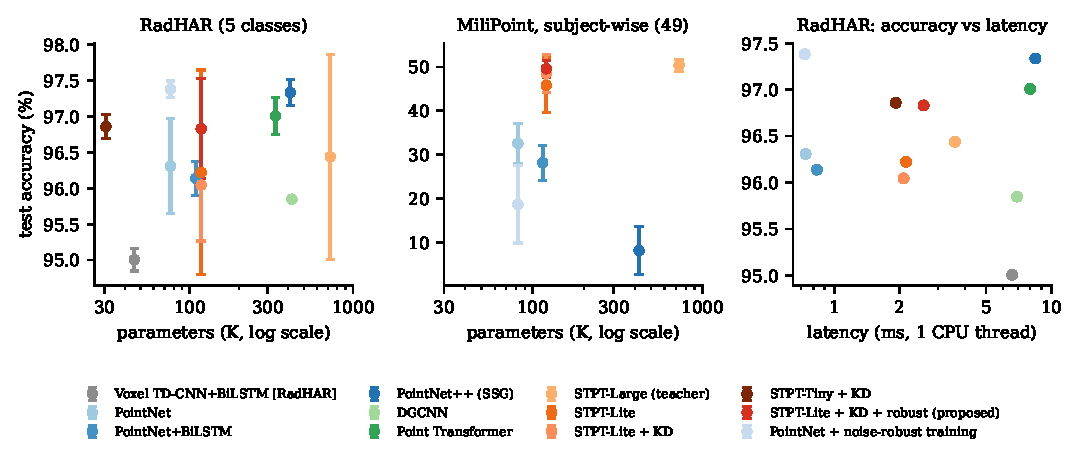
\includegraphics[width=\textwidth]{../figures/efficiency.pdf}
\caption{Accuracy (mean $\pm$ std over seeds) versus parameters on both datasets, and RadHAR accuracy versus single-thread CPU latency.}
\label{fig:efficiency}
\end{figure*}

\subsection{Ablation study}
\label{sec:ablation}
\begin{table}[t]
\centering
\caption{Ablation of STPT-Lite (no distillation): test accuracy (\%), mean\,$\pm$\,std over seeds (variants: 2 on RadHAR, 2 on MiliPoint; full model: 3), change w.r.t.\ the full model trained with the same seeds in brackets; $^\dagger$ single run.}
\label{tab:ablation}
\setlength{\tabcolsep}{3pt}
\resizebox{\columnwidth}{!}{%
\begin{tabular}{lcc}
\toprule
Variant & RadHAR & MiliPoint (subj.) \\
\midrule
STPT-Lite (full, no KD) & 96.22\,$\pm$\,1.43 & 45.79\,$\pm$\,6.30 \\
\midrule
-- intra-segment attention (max+attentive pool only) & 96.90\,$\pm$\,0.18 (+0.93) & 42.87\,$\pm$\,3.03 (-6.52) \\
-- motion descriptor & 97.67\,$\pm$\,0.16 (+1.70) & 49.90\,$\pm$\,2.06 (+0.50) \\
-- temporal Transformer (mean over segments) & 96.70\,$\pm$\,0.61 (+0.73) & 37.54\,$\pm$\,6.62 (-11.85) \\
-- Doppler \& intensity ($xyz$ only) & 96.42\,$\pm$\,1.69 (+0.45) & -- \\
-- spatial gating & 97.62\,$\pm$\,0.40 (+1.64) & -- \\
-- all training augmentation & 96.68\,$\pm$\,0.54 (+0.70) & -- \\
-- coordinate jitter augmentation & 95.86\,$\pm$\,1.13 (-0.11) & -- \\
\bottomrule
\end{tabular}}
\end{table}
Table~\ref{tab:ablation} removes one component of STPT-Lite (without
distillation) at a time and retrains with \ablSeeds{} seeds on RadHAR.
\textbf{MiliPoint (unseen people)} is the informative benchmark for the
architecture. Compared with the full model trained with the same two seeds
(49.4\% on average), removing the temporal Transformer (mean over segment
tokens instead) costs 11.9 points, and removing the intra-segment attention
(pooling only) costs 6.5 points. Both losses hold in each seed separately.
Fine-grained actions are therefore distinguished both by how the returns of a
short segment relate to each other and by how the segments evolve over the
window. The explicit motion descriptor brings no measurable gain (+0.5 points on
average, +2.8 and $-$1.8 in the two seeds): the attention layers apparently
recover centroid and displacement information from the point coordinates
themselves. We keep the descriptor because it costs only 2.5\,K parameters (2\% of the model), but
we do not claim it as a contribution to accuracy. \textbf{RadHAR} cannot rank
components. Every variant, including removing Doppler/intensity, gating or
augmentation, lies within about 1.7 points of the full model, inside its
seed spread ($\pm$1.4), because every model already exceeds 95\%. The
effect of the pre-processing is visible across models instead: with the same gating
and centring, all baselines exceed the published 90.47\%.


\subsection{Evaluation protocol and leakage}
\label{sec:protocol}
\begin{table}[t]
\centering
\caption{MiliPoint (49 actions) top-1 accuracy (\%) of the same models under three splits. Published numbers: 34.45 (PointNet++, \cite{cui2023milipoint}) and 98.25 (MAK-GCN, random 80/10/10, \cite{zakka2025makgcn}).}
\label{tab:protocol}
\setlength{\tabcolsep}{3pt}
\resizebox{\columnwidth}{!}{%
\begin{tabular}{lccc}
\toprule
Model & Subject-disjoint & Chronological & Random windows \\
 & (ours, primary) & (MiliPoint code) & (leaky) \\
\midrule
STPT-Lite & 45.79\,$\pm$\,6.30 & 58.38 (n=1) & 79.48 (n=1) \\
PointNet & 32.57\,$\pm$\,4.59 & 32.42 (n=1) & 44.44 (n=1) \\
\bottomrule
\end{tabular}}
\end{table}
The same STPT-Lite scores \mistptliteAcc\% under our subject-disjoint split,
\mpOfficialAcc\% under the chronological split of the MiliPoint code (which
shares subjects between training and test), and \mpRandomAcc\% under a random
split of overlapping windows (Table~\ref{tab:protocol}). The automated audit
explains this. Under the random split, \mpAuditLeakFrames\% of the test frames
also occur inside training windows, and \mpAuditLeakWins\% of the test windows
overlap a training window, by \mpAuditLeakOverlap\% of their length on average.
The inflation is therefore leakage, not learning. Accuracies of 98\% on
MiliPoint \cite{zakka2025makgcn} and ours of about 50\% describe different
tasks: recognising near-duplicates of seen sequences versus recognising actions
of new people. On RadHAR, the same audit found that every official test
recording lies within ten minutes of a training recording (median gap 29\,s) on
the same four days, and the dataset contains no subject identifiers. RadHAR
accuracy therefore measures generalisation to new recordings of known people
in a known room.

\subsection{Cross-dataset transfer}
\begin{table}[t]
\centering
\caption{Cross-dataset transfer (STPT-Lite, $xyz$ input): test accuracy (\%) when fine-tuning on a fraction of target training recordings/runs, from scratch vs.\ initialised from the model trained on the other dataset (mean\,$\pm$\,std, 3 seeds).}
\label{tab:transfer}
\setlength{\tabcolsep}{3pt}
\resizebox{\columnwidth}{!}{%
\begin{tabular}{llcc}
\toprule
Direction & Target data & Scratch & Pre-trained \\
\midrule
MiliPoint $\rightarrow$ RadHAR & 10\% & -- & -- \\
MiliPoint $\rightarrow$ RadHAR & 25\% & -- & -- \\
MiliPoint $\rightarrow$ RadHAR & 100\% & 95.23\,$\pm$\,0.00 & -- \\
\midrule
RadHAR $\rightarrow$ MiliPoint & 25\% & -- & -- \\
RadHAR $\rightarrow$ MiliPoint & 100\% & 45.79\,$\pm$\,6.30 & -- \\
\bottomrule
\end{tabular}}
\end{table}
Table~\ref{tab:transfer} initialises STPT-Lite from the MiliPoint model ($xyz$
input, harmonised axes) and fine-tunes it on a fraction of the RadHAR training
recordings. Pre-training on MiliPoint helps most when little RadHAR data is available. With
10\% of the RadHAR training recordings it raises test accuracy from
\trrhxyzscratchfTen\% to \trrhxyzmpinitfTen\% (two seeds; +18 points, larger
than the seed spread). With 25\% the gain shrinks to about one point, inside the
seed spread, and with all training data the pre-trained and scratch models are
equivalent (\trrhxyzmpinitfFull\% vs.\ \trrhablxyz\%). Since the two datasets
differ in radar, frame rate, subjects, room and label set, this suggests that
the segment tokenizer learns largely sensor-independent motion features from MiliPoint's
49 actions, which are most valuable when target labels are scarce, as in a new
home with few annotated recordings. With all data, one pre-trained seed reached its best validation score after the
first epoch and was stopped early (93.8\%); we report it unchanged.


\subsection{Noise robustness}
\begin{figure*}[t]
\centering
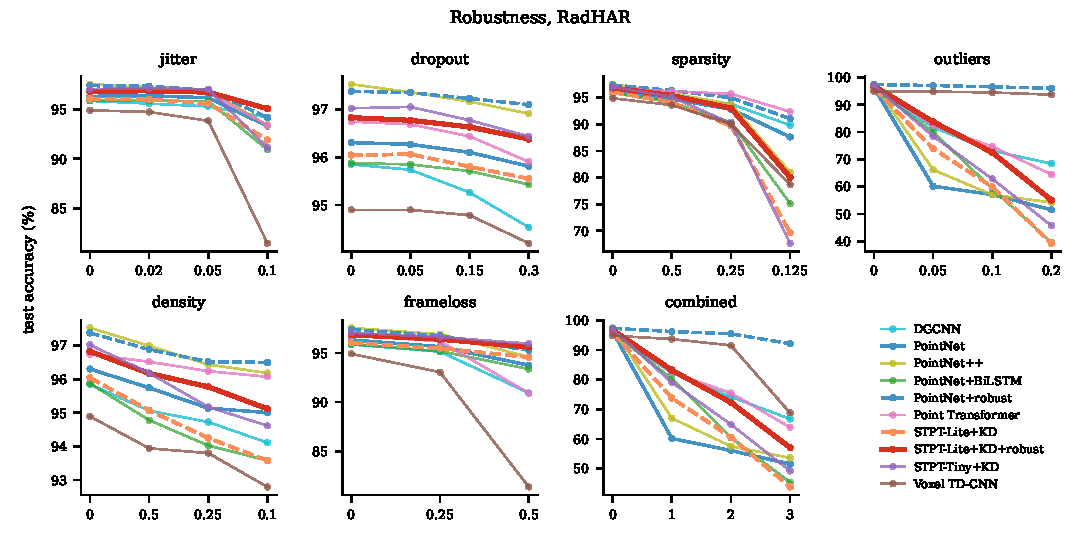
\includegraphics[width=0.49\textwidth]{../figures/robustness_radhar.pdf}\hfill
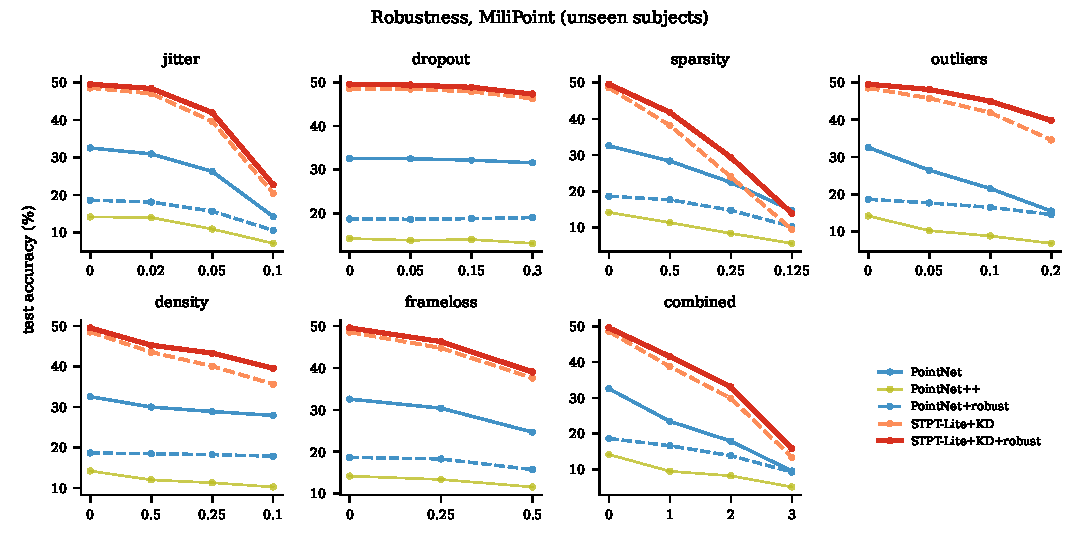
\includegraphics[width=0.49\textwidth]{../figures/robustness_milipoint.pdf}
\caption{Test accuracy under controlled perturbations (identical perturbed samples for every model; mean over the available seeds). Left: RadHAR; right: MiliPoint (unseen subjects).}
\label{fig:robust}
\end{figure*}
Fig.~\ref{fig:robust} reports test accuracy under seven perturbation types,
three severities each, applied with fixed seeds so that every model sees the
same perturbed windows. \textbf{MiliPoint (unseen people).} The proposed model
stays the most accurate under every condition except the most extreme
sparsity. Noise-robust training improves STPT-Lite+KD under all perturbations,
by 0.9--5.4 points (e.g.\ 20\% false detections: 34.6$\rightarrow$39.8\%; density
0.1: 35.6$\rightarrow$39.6\%), including jitter, which was not used in training
(22.8 vs.\ 20.5\% at $\sigma=10$\,cm). At 12.5\% of the returns kept (about one
point per frame), STPT-Lite (13.9\%) falls to the level of PointNet (14.7\%): with
almost no points per segment, intra-segment attention has nothing to attend to.
\textbf{RadHAR.} Dropout, density changes and jitter up to 5\,cm cost every
point-based model at most 2.5 points. Losing half of the segments costs DGCNN and
Point Transformer about five points but the proposed model only 1.2 points
(96.8$\rightarrow$95.6\%), which matches the even temporal attention in
Section~\ref{sec:xai}. Two conditions separate the
models. Under extreme sparsity, Point Transformer (92.4\%) and PointNet with
robust training (91.1\%) degrade least, the proposed model reaches 80.0\%, and
STPT-Lite+KD without robust training drops to 69.7\%. False detections are the
main weakness of the STPT family on RadHAR: at 20\% injected outliers the
proposed model keeps 55.1\% (39.3\% without robust training), whereas PointNet
with the same robust training keeps 96.0\% and the voxel CNN-LSTM 93.7\%.
A likely cause is that outliers corrupt the motion descriptor (centroid, mean Doppler) and receive
attention weight, while a max-pooled PointNet with robust training learns to
ignore isolated points and voxel occupancy dilutes them. Robust training
therefore helps, but it does not close this gap. A robust centroid (median) in
the motion descriptor and outlier-aware attention are the obvious next steps.


\subsection{Explainability and error analysis}
\label{sec:xai}
\begin{figure}[t]
\centering
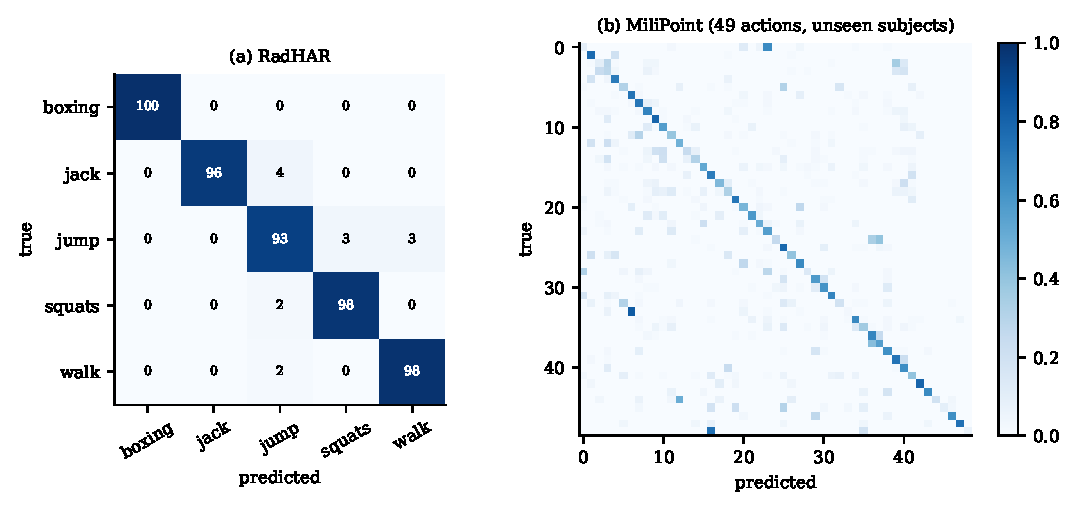
\includegraphics[width=\columnwidth]{../figures/confusion.pdf}
\caption{Row-normalised confusion matrices of the proposed STPT-Lite+KD+robust (seed 0).}
\label{fig:confusion}
\end{figure}
\begin{figure}[t]
\centering
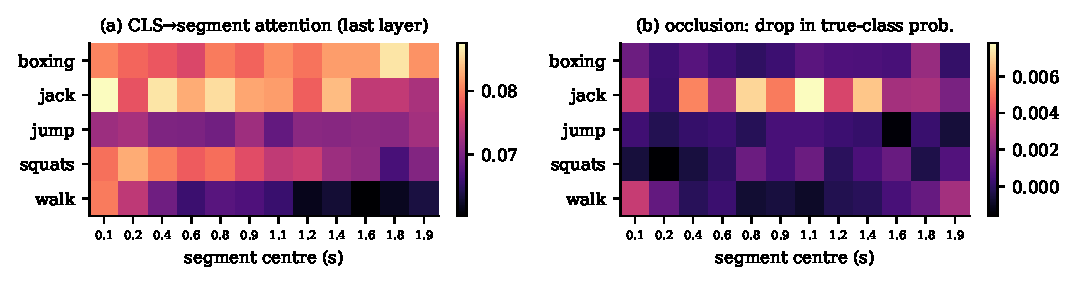
\includegraphics[width=\columnwidth]{../figures/xai_temporal.pdf}
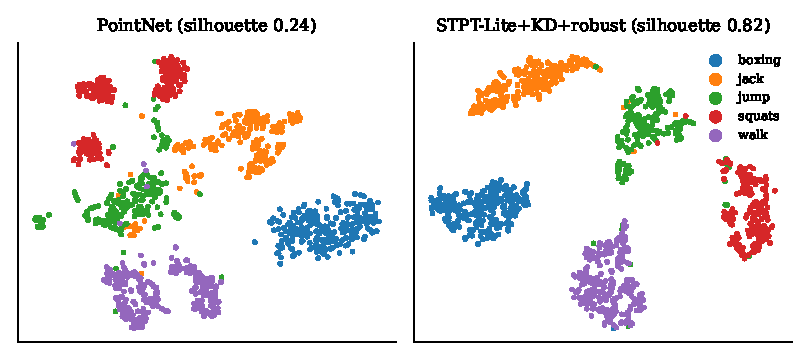
\includegraphics[width=\columnwidth]{../figures/tsne.pdf}
\caption{Top: mean [CLS]$\rightarrow$segment attention and segment-occlusion importance per class (RadHAR test). Bottom: t-SNE of test embeddings.}
\label{fig:xai}
\end{figure}
\textbf{Temporal attention and occlusion.} The [CLS] attention of the last
block is spread almost evenly over the twelve segments (0.07--0.09 per
segment, against 0.083 for uniform attention), with class-specific emphasis: the
middle of the window for jumping jacks, early segments for squats, and the
first segment for walking (Fig.~\ref{fig:xai}). Removing a single segment
(occlusion) lowers the true-class probability by less than one percentage point
on average. The model therefore integrates evidence over the whole window and
does not depend on any single 170-ms segment, which is consistent with its
tolerance to frame loss. Attention and occlusion importance agree only
moderately (Pearson $r=\xaiCorr$ over the class$\times$segment cells), so we
treat attention as a coarse indication and not as a faithful explanation.
\textbf{Point saliency.} Gradient saliency concentrates on the returns of the
moving limbs and torso and is low on isolated returns far from the body,
i.e.\ on the residual clutter that survives gating. \textbf{Embeddings.} In a
t-SNE of RadHAR test embeddings the classes form compact, well-separated
clusters (silhouette \silSTPTLiteKDrobust{} in the model's embedding space
versus \silPointNet{} for PointNet). \textbf{Errors.} The remaining RadHAR
errors are mostly windows predicted as \emph{jump} (precision 91\%), which
shares the strong vertical Doppler pattern of jumping jacks and squats. On
MiliPoint, errors concentrate in groups of kinematically similar actions.


\begin{table}[t]
\centering
\caption{Published results (as reported by the authors, under their own protocols; not directly comparable).}
\label{tab:sota}
\setlength{\tabcolsep}{3pt}
\resizebox{\columnwidth}{!}{%
\begin{tabular}{llrl}
\toprule
Method & Dataset & Acc. (\%) & Protocol / note \\
\midrule
TD-CNN+BiLSTM \cite{singh2019radhar} & RadHAR & 90.47 & official test, window-level val. \\
Lite-PointNet+BiLiLSTM \cite{gu2024lpn} & RadHAR & 95.12 & 79.7\,K params \\
GNN + 3-D joints \cite{lee2022gnn} & RadHAR & 96.55 & joint pre-training \\
MAK-GCN \cite{zakka2025makgcn} & RadHAR & 97.54 & 1.86\,M params \\
OG-PCL \cite{yan2025ogpcl} & RadHAR & 91.75 & 5-fold CV, 0.83\,M params \\
PointNet++ \cite{cui2023milipoint} & MiliPoint & 34.45 & chronological 80/10/10 \\
MAK-GCN \cite{zakka2025makgcn} & MiliPoint & 98.25 & random 80/10/10 \\
\midrule
STPT-Lite+KD+robust (ours) & RadHAR & \rastptlitekdrobustAcc & official test, recording-disjoint val. \\
STPT-Lite+KD+robust (ours) & MiliPoint & \mistptlitekdrobustAcc & subject-disjoint \\
\bottomrule
\end{tabular}}
\end{table}

\textbf{Published results.} Table~\ref{tab:sota} lists accuracies as reported by
other authors. They use different splits, pre-processing and training budgets
and are not directly comparable to ours; we include them for context only.
